\documentclass[a4paper,12pt]{article}
\usepackage{graphicx}
\usepackage{amsmath, amssymb, amsthm}
\usepackage{xcolor}
\definecolor{mydarkblue}{RGB}{0, 0, 139}
\usepackage[colorlinks=true, linkcolor=mydarkblue, citecolor=mydarkblue, urlcolor=mydarkblue]{hyperref}
\usepackage[english]{babel}
\usepackage[
  backend=biber,
  citestyle=authoryear,
  bibstyle=numeric,
  natbib=true,
  hyperref=true
]{biblatex}
\usepackage{amsfonts}
\usepackage{booktabs}
\usepackage{verbatim}

\title{{Wynn's $\rho$-Algorithm}}
\author{Lucas Posern}
\date{July 2025}
\addbibresource{quellen.bib}
\graphicspath{{figures/}}
\numberwithin{equation}{section}

% Reference commands
\newcommand{\secref}[1]{\hyperref[#1]{Section~\ref*{#1}}}
\newcommand{\figref}[1]{\hyperref[#1]{Figure~\ref*{#1}}}
\newcommand{\eqnref}[1]{\hyperref[#1]{Equation~\eqref{#1}}}
\newcommand{\lemref}[1]{\hyperref[#1]{Lemma~\ref*{#1}}}
\newcommand{\sref}[1]{\hyperref[#1]{Theorem~\ref*{#1}}}

\newtheorem{satz}{Theorem}[section]
\newtheorem{lemma}[satz]{Lemma}
\newtheorem{definition}[satz]{Definition}
\theoremstyle{remark}
\newtheorem*{bemerkung}{Remark}

\begin{document}
\maketitle
\thispagestyle{empty}
\newpage
\thispagestyle{empty}
\tableofcontents
\newpage
\pagenumbering{arabic} % start of arabic page numbering
\setcounter{page}{1}



\section{Introduction}\label{sec:einleitung}
General statements on convergence problems and their acceleration are taken from [\cite[194-199]{weniger1996nonlinear}].
Iterative methods play a central role in many areas of numerical mathematics and scientific computing. They serve to approximate solutions of equations, series or fixed-point problems step by step. A common problem of such methods, however, is their often slow convergence, which considerably increases the computational cost and limits efficiency and applicability in practice. This is where convergence acceleration comes in. It comprises methods that aim to improve the speed of approach to the limit significantly.

Wynn's $\rho$-algorithm, named after Peter Wynn, who developed it in the 1950s, is one of these methods for convergence acceleration. The algorithm originally arose from the challenge of improving the treatment of slowly convergent or even divergent series and sequences. In practice it turned out that many classical series expansions and iterative methods only yield usable results after a very large number of steps, provided they converge in finite time at all. The $\rho$-algorithm offers an elegant way of increasing the rate of convergence significantly by means of recursive transformations.

Wynn's $\rho$-algorithm is an extension of Wynn's $\epsilon$-algorithm. Although the two differ only slightly, this difference makes them applicable to different classes of convergence.

In the remainder of this work, Wynn's $\rho$-algorithm is presented in detail, its mathematical foundations are explained, and typical application examples are shown that illustrate its significance and performance in the field of convergence acceleration.

\section{The need for the $\rho$-algorithm}\label{sec:notwendigkeit}
For statements on Wynn's $\epsilon$-algorithm we refer to [\cite{wynn1966convergence}].\\

The $\epsilon$-algorithm, introduced by Peter Wynn (1956), was a major step forward for convergence acceleration thanks to its elegant recursion:
\[
\epsilon_{k+1}^{(n)} = \epsilon_{k-1}^{(n+1)} + \frac{1}{\epsilon_k^{(n+1)} - \epsilon_k^{(n)}}
\]
Nevertheless, the method has its limits:
\begin{enumerate}
\item \textbf{Not always successful}: For logarithmic convergence the $\epsilon$-algorithm fails.
\item \textbf{Rigid parameters}: The fixed coefficient structure ($+1$ in the numerator) does not allow any adaptation to different asymptotic expansions.
\end{enumerate}
The $\rho$-algorithm (Wynn, 1966) removes these deficiencies through a fundamental structural modification:
\[
\rho_{k+1}^{(n)} = \rho_{k-1}^{(n+1)} + \frac{k+1}{\rho_k^{(n+1)} - \rho_k^{(n)}}
\]
Its innovative power lies in the following core aspects:
\begin{enumerate}
\item \textbf{Acceleration for other sequences}: The $\rho$-algorithm succeeds in accelerating logarithmically convergent sequences by dynamically scaling the numerator with $k+1$.
\item \textbf{Parametrisability}: The extension to the $\rho(\gamma,p)$-algorithm (\secref{subsubsec:mod1}) allows adaptation to arbitrary expansions of the form $s_n \sim s + n^\theta(c_0 + c_1/n + \cdots)$.
\end{enumerate}

\section{Wynn's $\rho$-algorithm}\label{sec:wynn}
\subsection{Idea}\label{subsec:idee}

Wynn's $\rho$-algorithm is a technique for accelerating the convergence of numerical sequences. Especially for slowly convergent sequences, or for series whose sums are difficult to compute directly, the algorithm offers an effective way of improving numerical accuracy. It belongs to the so-called nonlinear transformations and is particularly suited to logarithmically convergent sequences.

The basic idea behind convergence acceleration methods is to generate, from a given sequence $\{s_n\}$, a new sequence $\{\rho_n\}$ that converges to the same limit, but considerably faster.

\subsection{Definition}\label{subsec:def}
We use the definition of the $\rho$-algorithm from [\cite[34-35]{weniger1996nonlinear}].\\
The $\rho$-algorithm is based on the recursive construction of a table, similar to the $\varepsilon$-algorithm. Given a sequence $\{s_n\}_{n=0}^{\infty}$, the rho table $\rho^{(k)}_n$ is defined recursively as follows:

\begin{align}
\rho^{(n)}_{-1} &= 0 \quad\\
\rho^{(n)}_0 &= s_n \\
\rho^{(n)}_{k+1} &= \rho^{(n+1)}_{k} + \frac{x_{n+k+1}-x_{n}}{\rho^{(n+1)}_{k} - \rho^{(n)}_k}, \quad k \ge 0 \label{eq:rhodef}
\end{align}
A prerequisite for the computation is that the interpolation points $x_n$ form an increasing divergent sequence:
\begin{gather*}
x_0<x_1<\cdots\\
\lim_{n\rightarrow\infty}x_{n}=\infty
\end{gather*}
In the case where the interpolation points simply correspond to the index of the sequence element ($x_n = n$), the algorithm can also be defined as:
\begin{align}
\rho^{(-1)}_n &= 0 \quad\\
\rho^{(0)}_n &= s_n \\
\rho^{(k+1)}_n &= \rho^{(k-1)}_{n+1} + \frac{k+1}{\rho^{(k)}_{n+1} - \rho^{(k)}_n}, \quad k \ge 0 \label{eq:rho_rek}
\end{align}
The value $\rho^{(2k)}_0$ yields the transformed approximation to the limit. The odd indices $\rho^{(2k+1)}_n$ are only of indirect significance for the approximation.

\subsection{Example}\label{subsec:beispiel}
As a simple example we consider the sequence
\begin{gather*}
s_n=\frac{2+3x_n}{1+x_n}, \quad x_n=n+1 \\
s=\lim_{n\rightarrow\infty}{s_n}=\lim_{n\rightarrow\infty}{\frac{2+3(n+1)}{1+(n+1)}}=3
\end{gather*}
The sequence elements are:
\begin{align*}
    s_0&=\frac{2+3x_n}{1+x_n}=\frac{2+3(0+1)}{1+(0+1)}=\frac{5}{2}=2.5\\
    s_1&=[...]=\frac{8}{3}\approx2.667\\
    s_2&= [...]=2.75\\
    s_3&= [...]=2.8
\end{align*}
$\rho$-iterations:
\begin{align*}
    \rho_{-1}^{(n)}&=0\\
    \rho_{0}^{(n)}&=s_n\\
    \rho_{k+1}^{(n)}&=\rho_{k-1}^{(n+1)}+\frac{x_{n+k+1}-x_{n}}{\rho_{k}^{(n+1)}-\rho_{k}^{(n)}}
\end{align*}
Fill in the $\rho$ table:
\begin{table}[h!]
\centering
\begin{tabular}{c@{\hspace{1.5cm}}c@{\hspace{1.5cm}}c}
$n$ & $\rho_{-1}^{(n)}$ & $\rho_{0}^{(n)}$ \\
\midrule
    0 & 0 & 2.500 \\
    1 & 0 & 2.667 \\
    2 & 0 & 2.750 \\
    3 & 0 & 2.800 \\
\end{tabular}
\end{table}
\\\\
Stage 1, k=0: $\rho_{1}^{(n)}=\rho_{-1}^{(n+1)}+\frac{x_{n+1}-x_{n}}{\rho_{0}^{(n+1)}-\rho_{0}^{(n)}}$
\begin{align*}
    \rho_{1}^{(0)}&=0+\frac{x_{1}-x_{0}}{s_1-s_{0}}=\frac{2-1}{2.667-2.500}=\frac{1}{0.1667}\approx6\\
    \rho_{1}^{(1)}&=0+\frac{x_{2}-x_{1}}{s_2-s_{1}}=\frac{3-2}{2.750-2.667}=\frac{1}{0.0833}\approx12\\
    \rho_{1}^{(2)}&=0+\frac{x_{3}-x_{2}}{s_3-s_{2}}=\frac{4-3}{2.800-2.750}=\frac{1}{0.05}=20
\end{align*}
Stage 2, k=1: $\rho_{2}^{(n)}=\rho_{0}^{(n+1)}+\frac{x_{n+1+1}-x_{n}}{\rho_{1}^{(n+1)}-\rho_{1}^{(n)}}$
\begin{align*}
    \rho_{2}^{(0)}&=s_1+\frac{x_{2}-x_{0}}{\rho_1^{(1)}-\rho_1^{(0)}}=2.667+\frac{3-1}{12-6}=2.667+\frac{2}{6}\approx3\\
    \rho_{2}^{(1)}&=s_2+\frac{x_{3}-x_{1}}{\rho_1^{(2)}-\rho_1^{(1)}}=2.750+\frac{4-2}{20-12}=2.750+\frac{2}{8}=3
\end{align*}
The $\rho$ table now reads:
\begin{table}[h!]
\centering
\begin{tabular}{c@{\hspace{1.1cm}}c@{\hspace{1.1cm}}c@{\hspace{1.1cm}}c@{\hspace{1.1cm}}c}
$n$ & $\rho_{-1}^{(n)}$ & $\rho_{0}^{(n)}$ & $\rho_{1}^{(n)}$ & $\rho_{2}^{(n)}$\\
\midrule
    0 & 0 & 2.500 & 6 & 3\\
    1 & 0 & 2.667 & 12 & 3\\
    2 & 0 & 2.750 & 12\\
    3 & 0 & 2.800 \\
\end{tabular}
\end{table}
\\
$\implies$ The acceleration was successful.\\\\
The transformed values $\rho_{2}^{(0)}$ and $\rho_{2}^{(1)}$ coincide with the limit $s=3$. This is a strong improvement in the acceleration of convergence.

\subsection{Acceleration}\label{subsec:beweis}
The proof that the $\rho$-algorithm accelerates a sequence is taken from [\cite[522-525]{osada1996acceleration}].\\
In this work we prove that the $\rho$-algorithm accelerates the convergence of a sequence
\[
s_n \sim s + n^{\theta}(c_0  + \frac{c_1}{n} + \frac{c_2}{n^2} + \dots) \quad \text{as } n \to \infty
\]
if and only if $\theta$ is a negative integer. We also show that the $\rho$-algorithm cannot accelerate linear convergence.

\begin{definition}[Associated sequence]\label{subsec:assoz}
\textnormal{To describe the asymptotic behaviour of the $\rho$-algorithm, we use a related sequence.} For given $\theta \notin \big\{0,1\big\}$ and given $c \ne 0$ we define a sequence $(C_k)_{k=-1,0,1,\dots}$ by:
\begin{align*}
C_{-1} &= 0 \\
C_0 &= c \\
C_{2k-1} &= C_{2k-3} + \frac{2k - 1}{\theta C_{2k-2}}, \quad k = 1, 2, \dots\\
C_{2k} &= C_{2k-2} + \frac{2k}{(1 - \theta) C_{2k-1}}, \quad k = 1, 2, \dots
\end{align*}
We call this sequence $(C_k)$ the associated sequence of the $\rho$-algorithm with respect to $\theta$ and $c$.
\end{definition}

\begin{lemma}\label{lemma}
The associated sequence can be represented explicitly as
\[
C_{2k-1} =
\begin{cases}
\frac{1}{c\theta}, & k = 1, \\
\frac{k(2-\theta)\cdots(k-\theta)}{c\theta(1+\theta)\cdots(k-1+\theta)}, & k > 1,
\end{cases}
\]
\[
C_{2k} = \frac{c(1+\theta)\cdots(k+\theta)}{(1-\theta)\cdots(k-\theta)},
\]
where
\[
k \in
\begin{cases}
k\in\mathbb{N}, & \theta \notin \mathbb{Z}, \\
k< \theta, & \theta \in \mathbb{N}, \\
k\leq |\theta|, & -\theta \in \mathbb{N}.
\end{cases}
\]
\end{lemma}

\begin{proof}
The proof is by induction. The representations are true for $k = 1$, because
\[
C_1 = C_{-1} + \frac{1}{c\theta} = \frac{1}{c\theta}, \quad \text{and} \quad
C_2 = C_0 + \frac{2}{(1-\theta)C_1} = \frac{c(1+\theta)}{1-\theta}.
\]
Assume they hold for $k > 1$. By the induction hypothesis we obtain
\begin{align*}
C_{2k+1} &= C_{2k-1} + \frac{2k + 1}{\theta C_{2k}} \\
&= \frac{k(2-\theta)\cdots(k-\theta)}{c\theta(1+\theta)\cdots(k+\theta)}
+ \frac{(2k+1)(1-\theta)\cdots(k-\theta)}{c\theta(1+\theta)\cdots(k-1+\theta)} \\
&= \frac{(k+1)(2-\theta)\cdots(k-\theta)(k+1-\theta)}{c\theta(1+\theta)\cdots(k+\theta)}.
\end{align*}
Likewise,
\[
C_{2k+2} = \frac{c(1+\theta)(2+\theta)\cdots(k+1+\theta)}{(1-\theta)\cdots(k+1-\theta)}.
\]

\end{proof}

\begin{satz}\label{satz1}
Let \((s_n)\) be a sequence with
\[
s_n \sim s + n^{\theta} \left( c_0 + \frac{c_1}{n} + \frac{c_2}{n^2} + \cdots \right), \quad n \to \infty
\]
\textit{with \(\operatorname{Re} \theta < 0\), \(c_0 \neq 0\) and constants \(c_k\). Let \((C_k)\) be the associated sequence for \(\theta\) and \(c_0\), and}
\[
A = (1 - \theta) \left( -\frac{1}{2} + \frac{c_1}{c_0 \theta} \right).
\]
\textit{Then, for fixed \(k \in \mathbb{N}\) with \(\theta \neq -1, \dots, 1 - k\):}
\begin{align*}
\rho_{2k-1}^{(n)} &= C_{2k-1} (n + k)^{1 - \theta} \left( 1 + \frac{A}{n + k} \right) + O\left( (n + k)^{-1 - \theta} \right), \\
\rho_{2k}^{(n)} &= s + C_{2k} (n + k)^{\theta} \left( 1 + \frac{c_1}{c_0 (n + k)} \right) + O\left( (n + k)^{\theta - 2} \right).
\end{align*}
\end{satz}
\begin{proof}
We proceed by induction on \(k\).

\paragraph{Base case (\(k = 1\)):}
For \(\rho_1^{(n)}\) and \(\rho_2^{(n)}\) we use the definition of the \(\rho\)-algorithm:
\[
\rho_1^{(n)} = n + \frac{1}{s_{n+1} - s_n}, \quad
\rho_2^{(n)} = s_{n+1} + \frac{2}{(s_{n+2} - s_{n+1})^{-1} - (s_{n+1} - s_n)^{-1}}.
\]
Using the asymptotic expansion of \(s_n\) and a binomial expansion we obtain:
\[
s_{n+1} - s_n = c_0 \theta (n + 1)^{\theta - 1} \left[ 1 - \frac{A}{n + 1} + \kappa_1 (n + 1)^{-2} + O\left( (n + 1)^{\theta - 3} \right) \right],
\]
where \(\kappa_1 = -\frac{(1 - \theta)(2 - \theta)}{12} + \frac{c_1 (1 - \theta)}{2c_0} + \frac{c_2}{c_0 \theta}\). Substituting into \(\rho_1^{(n)}\) yields:
\[
\rho_1^{(n)} = \frac{1}{c_0 \theta} (n + 1)^{1 - \theta} \left[ 1 + \frac{A}{n + 1} + \kappa_2 (n + 1)^{-2} + O\left( (n + 1)^{-3} \right) \right] + n,
\]
with \(\kappa_2 = A^2 - \kappa_1\). Since \(C_1 = \frac{1}{c_0 \theta}\) (from \lemref{lemma}) and \((n + 1)^{1 - \theta}\) dominates \(n\) for \(\operatorname{Re} \theta < 0\), it follows that:
\[
\rho_1^{(n)} = C_1 (n + 1)^{1 - \theta} \left( 1 + \frac{A}{n + 1} \right) + O\left( (n + 1)^{-1 - \theta} \right).
\]
Analogously one shows for \(\rho_2^{(n)}\):
\[
\rho_2^{(n)} = s + C_2 (n + 1)^{\theta} \left( 1 + \frac{c_1}{c_0 (n + 1)} \right) + O\left( (n + 1)^{\theta - 2} \right),
\]
where \(C_2 = \frac{c_0 (1 + \theta)}{1 - \theta}\) (\lemref{lemma}).

\paragraph{Induction step (\(k \to k + 1\)):}
Assumption: the statements hold for an arbitrary \(k \geq 1\).

\begin{enumerate}
\item {Show \(\rho_{2k+1}^{(n)}\):} \\
By the definition of the \(\rho\)-algorithm:
\[
\rho_{2k+1}^{(n)} = \rho_{2k-1}^{(n+1)} + \frac{2k + 1}{\rho_{2k}^{(n+1)} - \rho_{2k}^{(n)}}.
\]
From the induction hypothesis for \(\rho_{2k}^{(m)}\) it follows that:
\[
\rho_{2k}^{(n+1)} - \rho_{2k}^{(n)} = \theta C_{2k} (n + k + 1)^{\theta - 1} \left[ 1 - \frac{A}{n + k + 1} \right] + O\left( (n + k + 1)^{\theta - 3} \right).
\]
For \(\rho_{2k-1}^{(n+1)}\) we have:
\[
\rho_{2k-1}^{(n+1)} = C_{2k-1} (n + k + 1)^{1 - \theta} \left( 1 + \frac{A}{n + k + 1} \right) + O\left( (n + k + 1)^{-1 - \theta} \right).
\]
Substituting and rearranging gives:
\[
\rho_{2k+1}^{(n)} = \underbrace{C_{2k-1} + \frac{2k + 1}{\theta C_{2k}}}_{= C_{2k+1} \text{ (recursion from \lemref{lemma})}} (n + k + 1)^{1 - \theta} \left( 1 + \frac{A}{n + k + 1} \right) + R_n,
\]
where the remainder \(R_n = O\left( (n + k + 1)^{-1 - \theta} \right)\) absorbs all errors. Hence:
\[
\rho_{2k+1}^{(n)} = C_{2k+1} (n + k + 1)^{1 - \theta} \left( 1 + \frac{A}{n + k + 1} \right) + O\left( (n + k + 1)^{-1 - \theta} \right).
\]

\item {Show \(\rho_{2k+2}^{(n)}\):} \\
Analogously:
\[
\rho_{2k+2}^{(n)} = \rho_{2k}^{(n+1)} + \frac{2k + 2}{\rho_{2k+1}^{(n+1)} - \rho_{2k+1}^{(n)}}.
\]
From what has just been shown it follows that:
\[
\rho_{2k+1}^{(n+1)} - \rho_{2k+1}^{(n)} = (1 - \theta) C_{2k+1} (n + k + 1)^{-\theta} \left[ 1 - \frac{c_1}{c_0 (n + k + 1)} \right] + O\left( (n + k + 1)^{-2 - \theta} \right).
\]
With the induction hypothesis for \(\rho_{2k}^{(n+1)}\) we obtain:
\[
\rho_{2k}^{(n+1)} = s + C_{2k} (n + k + 1)^{\theta} \left( 1 + \frac{c_1}{c_0 (n + k + 1)} \right) + O\left( (n + k + 1)^{\theta - 2} \right).
\]
Substituting and using the recursion \(C_{2k+2} = C_{2k} + \frac{2k + 2}{(1 - \theta) C_{2k+1}}\) (\lemref{lemma}) yields:
\[
\rho_{2k+2}^{(n)} = s + C_{2k+2} (n + k + 1)^{\theta} \left( 1 + \frac{c_1}{c_0 (n + k + 1)} \right) + O\left( (n + k + 1)^{\theta - 2} \right). \qedhere
\]
\end{enumerate}

\end{proof}




\begin{satz}[Acceleration]\label{satz2}
\textit{Let $(s_n)$ be a sequence with
\[
s_n \sim s + n^{\theta}(c_0 + \frac{c_1}{n} + \frac{c_2}{n^2} + \cdots), \quad \text{as } n \to \infty
\]
with $c_0 \ne 0$.
The $\rho$-algorithm accelerates the convergence of the sequence $(s_n)$ if and only if $\theta$ is a negative integer.}
\end{satz}

\begin{proof}
By \sref{satz1} we have, for every fixed $k$:
\begin{align*}
\lim_{n \to \infty} \frac{\rho_{2k}^{(n)} - s}{s_{n+2k} - s} &= \lim_{n \to \infty}\frac{s+C_{2k}(n+k)^{\theta}(1+\frac{c_0}{c_1(n+k)})+O((n+k)^{\theta-2})-s}{s+(n+2k)^\theta(c_0+\frac{c_1}{n+2k}+\frac{c_2}{(n+2k)^2}+\dots)-s}\\
&=\lim_{n \to \infty}\frac{C_{2k}(n+k)^{\theta}(1+\frac{c_0}{c_1(n+k)})+O((n+k)^{\theta-2})}{(n+2k)^\theta c_0(1+\frac{c_1}{c_0(n+2k)}+\frac{c_2}{c_0(n+2k)^2}+\dots)}\\
&=\frac{C_{2k}}{c_0}
\end{align*}
In the general case $\frac{C_{2k}}{c_0}\neq0$ and the algorithm does not converge faster than the original sequence. By \lemref{lemma}, however, we know:

\begin{center}
$\theta = -k$ for $k \in \mathbb{N}$ $\implies$ $C_0\ne0,\dots,C_{2k-2}\ne0$ and $C_{2k} = 0$
\end{center}
It follows immediately that $\lim_{n \to \infty} \frac{\rho_{2k}^{(n)} - s}{s_{n+2k} - s}=\frac{C_{2k}}{c_0}=0$. Hence the $\rho$-algorithm accelerates the sequence $s_n$.

\end{proof}




\subsection{Weaknesses}\label{subsec:schwächen}
For the following two theorems we refer to [\cite[526-527]{osada1996acceleration}]. They are applied only to definition \eqref{eq:rho_rek} (numerator $= k+1$).
\begin{satz}\label{satz3}
\textnormal{Here we use an alternative definition of linear convergence.}
\textit{Let $(s_n)$ be a sequence converging to $s$ with $e_n = s_n - s$, where
\[
e_{n+1} = (\lambda + \varepsilon_n)e_n, \quad \lambda\in[-1,1)\setminus\{0\}, \space \varepsilon_n \to 0.
\]
Then
\[
\rho^{(n)}_{2k} = s + (-1)^k e_{n+k} + O(e_{n+k} \varepsilon_{n,k-1}),
\]
with $\varepsilon_{n,k} = \max\{ |\varepsilon_n|, \ldots, |\varepsilon_{n+k}| \}$.}
\end{satz}
\begin{proof}
The proof can be found in [\cite[526-527]{osada1996acceleration}]. The idea of the proof is to first define a recursive, alternating sequence $D_k$ and then to show by induction that the $\rho$-algorithm can be represented in terms of this sequence.
\end{proof}

\begin{satz}\label{satz4}
\textit{The $\rho$-algorithm cannot accelerate linear convergence.}
\end{satz}

\begin{proof}
By \sref{satz3} we obtain:
\begin{align*}
    \lim_{n \to \infty} \frac{ \rho^{(n)}_{2k} - s }{ s_{n+2k} - s } &= \lim_{n \to \infty} \frac{ s + (-1)^k e_{n+k} + O(e_{n+k} \varepsilon_{n,k-1}) - s }{ s + e_{n+2k} - s } \\
&=\lim_{n \to \infty} \frac{(-1)^k e_{n+k} + O(e_{n+k} \varepsilon_{n,k-1})}{e_{n+2k}} \\
&=\frac{(-1)^k\lambda^k e_{n}}{\lambda^{2k}e_{n}} \\
&=\frac{(-1)^k}{\lambda^k} \ne 0.
\end{align*}
Hence no acceleration is achieved.

\end{proof}
\newpage
\section{Examples, tests \& comparisons with other methods}\label{sec:beispiele}

\subsection{Linearly convergent sequences: comparison of $\rho$ and Aitken's $\Delta^2$}\label{subsec:linear}
The following statement on Aitken's $\Delta^2$ method is found in [\cite[2]{pomeranz2017aitken}].
In \secref{subsec:schwächen} we proved that the $\rho$-algorithm does not accelerate linearly convergent sequences. The figure below shows the same thing by example. We compare Aitken's $\Delta^2$ method, which accelerates linearly convergent sequences with high efficiency, against the $\rho$-algorithm:\\
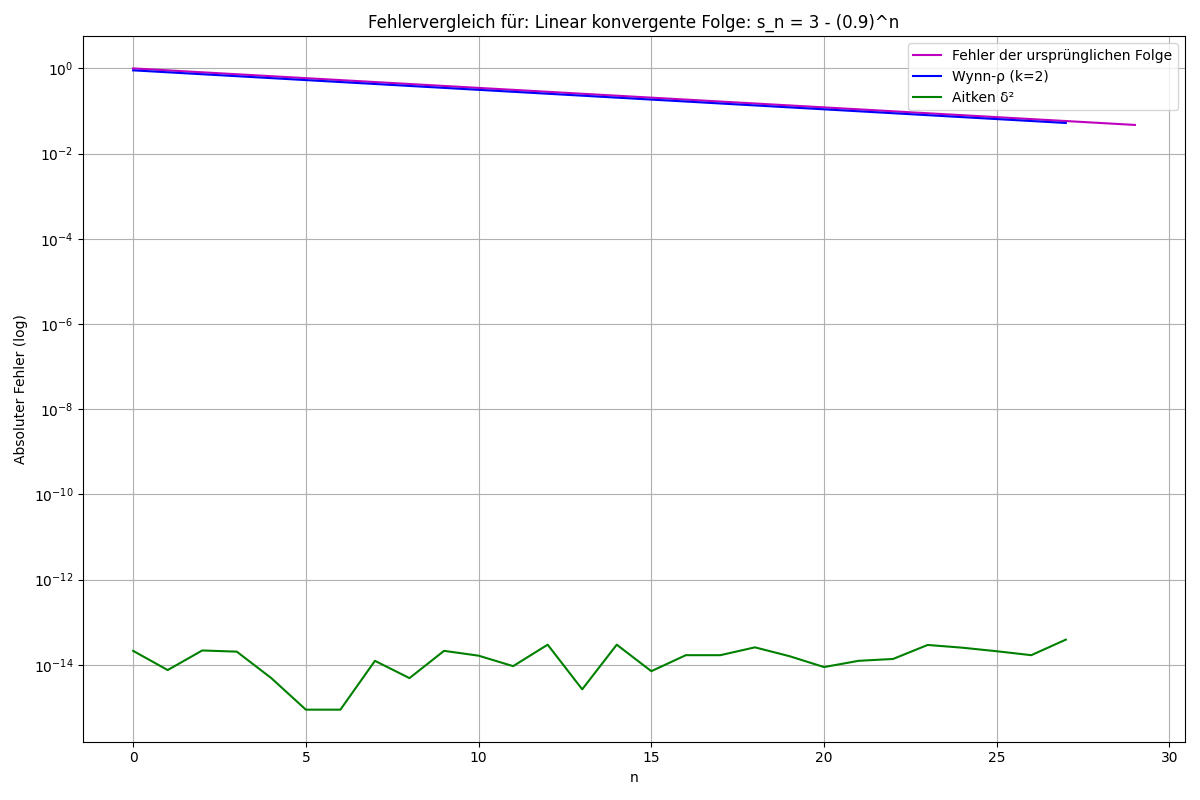
\includegraphics[width=\textwidth]{aitkenvsrho.png}\\
While the error of Aitken's $\Delta^2$ method becomes very small very quickly, the error of the $\rho$ sequence behaves exactly like the error of the original sequence $s_n$.

\newpage
\subsection{Alternating sequences: comparison of $\rho$ and $\epsilon$}\label{subsec:alternierend}
The strengths and weaknesses of the $\epsilon$-algorithm are discussed in more detail in [\cite[112-115]{wynn1966convergence}]. The $\epsilon$-algorithm is particularly efficient at accelerating alternating sequences. The $\rho$-algorithm yields hardly any improvement here. To see this, we consider the Leibniz series and compare the $\epsilon$-algorithm with the $\rho$-algorithm:
\[
\sum_{k=0}^{\infty} (-1)^k \frac{1}{2k + 1} = \frac{\pi}{4}
\]
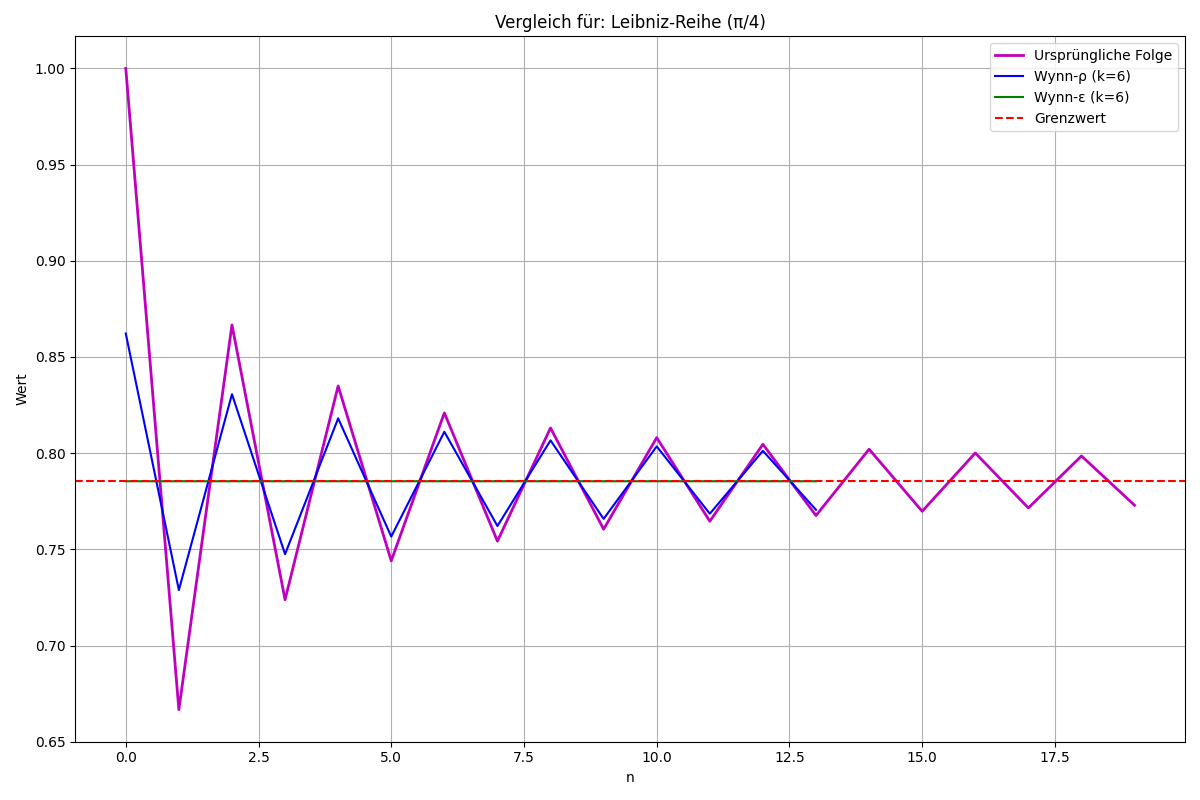
\includegraphics[width=\textwidth]{epsilonvsrho.png}
\\
The $\epsilon$-algorithm already achieves a very accurate value at $n=0$, whereas the $\rho$-algorithm merely approaches the original sequence.

\newpage
\subsection{Logarithmically convergent sequences}\label{subsec:log}
The $\rho$-algorithm shows its particular strength in accelerating logarithmically convergent sequences. We consider the so-called $Euler$-$Mascheroni$ $constant$, which is described by
\[
\lim_{n \to \infty}\sum\limits_{k=1}^{n}\frac{1}{k}-ln(n) \approx0.57721566
\]
We do not use a figure here, since we only want to analyse the accuracy of the $\rho$-algorithm. The algorithm produces the following values:\\\\
\begin{tabular}{c|r|r|r|r|r}
$n$ & $k=-1$ & $k=0$ & $k=2$ & $k=4$ & $k=6$ \\
\hline
0 & 0.00000000 & 1.00000000 & 0.\underline{57}660033 & 0.\underline{5772}8341 & 0.\underline{577215}75 \\
1 & 0.00000000 & 0.80685282 & 0.\underline{57}692144 & 0.\underline{5772}2282 & 0.\underline{5772156}7 \\
2 & 0.00000000 & 0.73472104 & 0.\underline{577}06845 & 0.\underline{5772}1759 & 0.\underline{57721566} \\
3 & 0.00000000 & 0.69703897 & 0.\underline{577}13320 & 0.\underline{5772}1638 & 0.\underline{57721566} \\
4 & 0.00000000 & 0.67389542 & 0.\underline{577}16520 & 0.\underline{577215}98 & 0.\underline{57721566} \\
5 & 0.00000000 & 0.65824053 & 0.\underline{577}18265 & 0.\underline{577215}82 & 0.\underline{57721566} \\
6 & 0.00000000 & 0.64694699 & 0.\underline{577}19292 & 0.\underline{577215}75 & 0.\underline{57721566} \\
7 & 0.00000000 & 0.63841560 & 0.\underline{577}19935 & 0.\underline{577215}72 & 0.\underline{57721566} \\
8 & 0.00000000 & 0.63174368 & 0.\underline{5772}0357 & 0.\underline{577215}70 & 0.\underline{57721566} \\
9 & 0.00000000 & 0.62638316 & 0.\underline{5772}0646 & 0.\underline{577215}69 & 0.\underline{57721566} \\
10 & 0.00000000 & 0.62198207 & 0.\underline{5772}0850 & 0.\underline{577215}68 & 0.\underline{57721566} \\

\end{tabular}\\\\\\
We therefore reach the exact result already at recursion step $k=6$ with depth $n=2$.




\newpage
\subsection{Slowly convergent sequences}\label{subsec:langsam}
The behaviour of the $\rho$-algorithm when applied to the zeta function is equally interesting:
\[
\zeta(s) = \sum_{n=1}^{\infty} \frac{1}{n^s}
\]
This converges particularly slowly when $s\downarrow1$. We therefore compare the $\rho$-algorithm with the $\epsilon$-algorithm, which has great difficulty here. In the figure, $s=1.5$ is the example value.\\\\
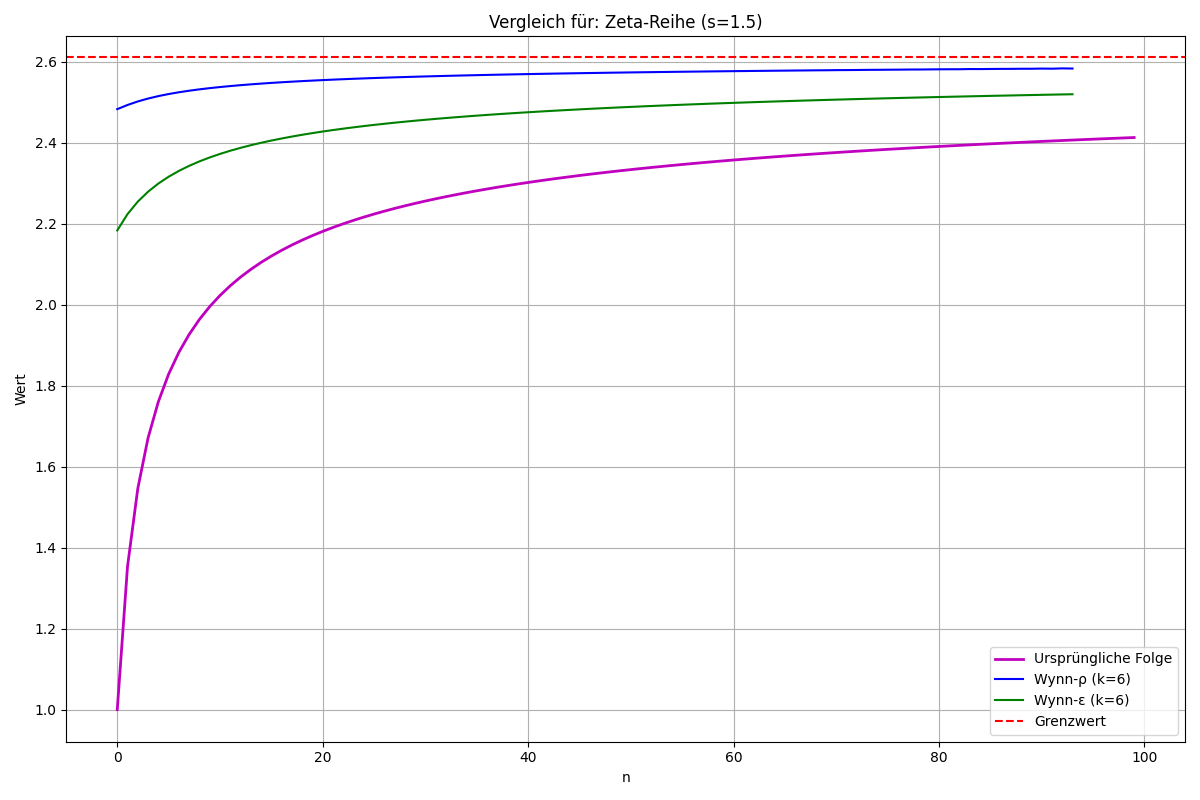
\includegraphics[width=\textwidth]{zetaepsvsrho.png}
\\
The $\rho$-algorithm still performs well by comparison, but the acceleration already costs it more effort here. As $s$ approaches $1$, the efficiency of the algorithm decreases further. We address this problem in \secref{subsubsec:mod1}.

\newpage
\subsection{Modifications}\label{subsec:modifikationen}
For the following two modifications we refer to [\cite[376-378]{sidi2003practical}]; the text below only gives the definitions together with one application example each.\\
By slightly changing the original definition we can achieve very strong improvements in some cases. In essence, we change the term that describes the interpolation points in the classical definition \eqref{eq:rhodef}, which are defined as $(k+1)$ by default.
\subsubsection{Modification 1: the $\rho(\gamma)$-algorithm}\label{subsubsec:mod1}
We define the $\rho(\gamma)$-algorithm as
\begin{align*}
\overline\rho^{(n)}_{-1} &= 0 \quad\\
\overline\rho^{(n)}_0 &= s_n \\
\overline\rho^{(n)}_{k+1} &= \overline\rho^{(n+1)}_{k-1} + \frac{k - \gamma}{\overline\rho^{(n+1)}_{k} - \overline\rho^{(n)}_k}
\end{align*}
\subsubsection*{Leibniz series}
If we now apply this algorithm with a suitable $\gamma$ to the $Leibniz$ $series$, we achieve a strong improvement in convergence compared with the classical algorithm. To this end we consider the example of the alternating harmonic series:\\
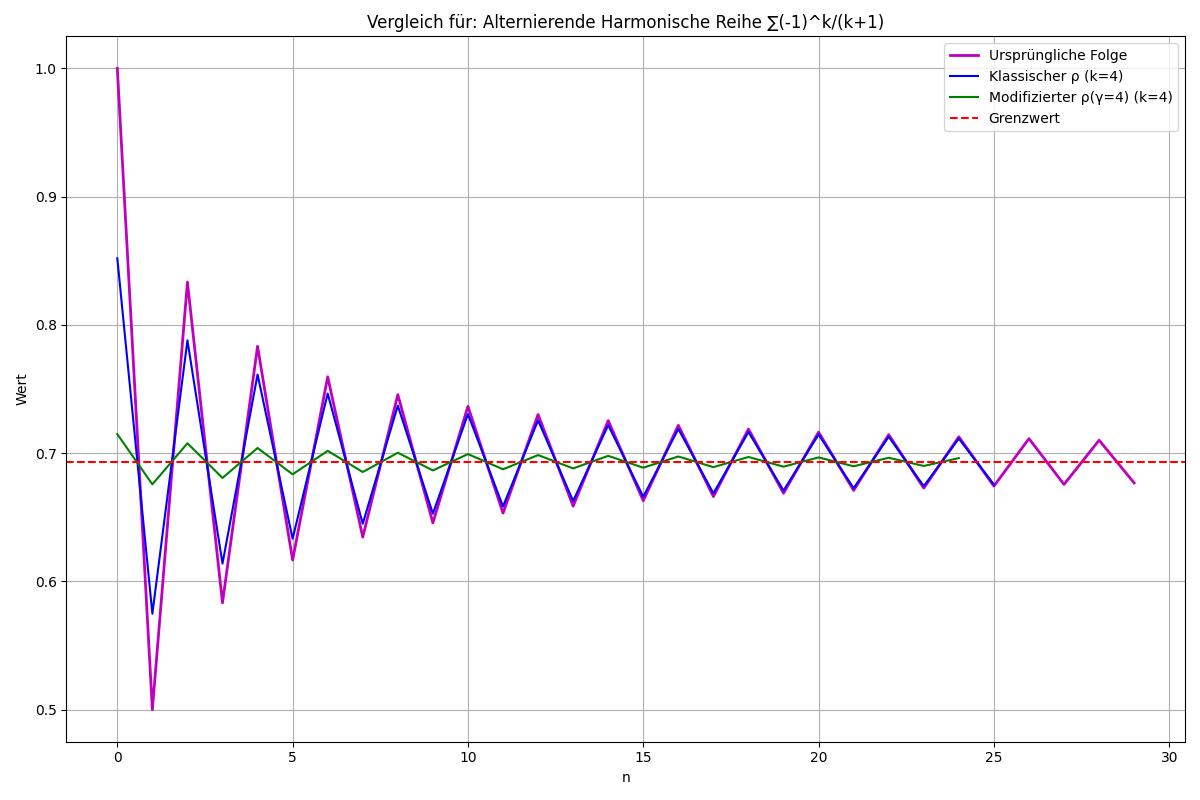
\includegraphics[width=\textwidth]{modi1.png}
We see a very strong improvement compared with the original algorithm. If we choose $\gamma$ even larger, we approach the actual limit ever more closely.
\subsubsection*{Zeta function}
In \secref{subsec:langsam} we already observed a limited acceleration for the zeta function by the $\rho$-algorithm. With a suitable choice of parameters, however, we can optimise this.\\\\
The exact value is
\[
\zeta(1.1)=10.58444846
\]
Whereas the classical $\rho$-algorithm still has an error of $(e_{23}>5)$ at a recursion depth of $n=23$, our modified $\rho(\gamma)$-algorithm with the parameter $\gamma=0.9$ achieves an error of $(e_{23}^{\gamma}\approx10^{-8})$.

The parameter has to be chosen very carefully here; small deviations can ruin the acceleration completely in this case.\\
\begin{center}
\begin{tabular}{c|c|c|c}
$n$ & Original & $\rho$ (standard)& $\rho(\gamma=0.9)$ \\ \hline
0 & 1.00000000 & 4.05905983 & \underline{10.584}39421 \\
1 & 1.46651650 & 4.21881639 & \underline{10.5844}2870 \\
2 & 1.76516932 & 4.34421820 & \underline{10.5844}3969 \\
3 & 1.98280696 & 4.44700181 & \underline{10.58444}402 \\
4 & 2.15307494 & 4.53383717 & \underline{10.58444}598 \\
5 & 2.29240141 & 4.60885546 & \underline{10.58444}697 \\
6 & 2.40999730 & 4.67478432 & \underline{10.58444}752 \\
7 & 2.51152885 & 4.73351524 & \underline{10.58444}784 \\
8 & 2.60072236 & 4.78641165 & \underline{10.584448}03 \\
9 & 2.68015518 & 4.83448760 & \underline{10.584448}16 \\
10 & 2.75168186 & 4.87851702 & \underline{10.584448}24 \\
11 & 2.81667995 & 4.91910356 & \underline{10.584448}30\\
12 & 2.87619987 & 4.95672683 & \underline{10.584448}34 \\
13 & 2.93106029 & 4.99177397 & \underline{10.584448}37 \\
14 & 2.98191131 & 5.02456188 & \underline{10.584448}39 \\
... & ... & ... & ... \\
23 & 3.32204995 & 5.25044529 & \underline{10.5844484}5
\end{tabular}
\end{center}
\subsubsection{Automated $\rho(\gamma)$-algorithm}
The following gives a brief insight into a possible automation of the $\rho(\gamma)$ method. Further details on the automation and on the connection to other acceleration methods can be found in [\cite[378]{sidi2003practical}].

The automated $\rho(\gamma)$-algorithm accelerates the convergence of sequences $\{s_n\}$ by adaptive parameter estimation.\\\\
The idea is that for sequences with asymptotic behaviour
\[ s_n \sim s + \sum_{i=0}^\infty \alpha_i n^{\gamma-i} \quad (n\to\infty) \]
the algorithm automatically determines the optimal parameter $\gamma'$ and applies the $\rho(\gamma')$-algorithm.

\subsubsection*{Algorithm}
\begin{enumerate}
\item {Parameter estimation}:
\begin{itemize}
\item Input: $s_0,\ldots,s_r$
\item Apply the $\rho(-2)$-algorithm to the auxiliary sequence $\{\gamma_m\}_{m=0}^{r-2}$
\item Set:
  \[ \gamma' = \begin{cases}
  \bar{\rho}_{2k}^{(0)} & \text{for } r=2k+2 \\
  \bar{\rho}_{2k}^{(1)} & \text{for } r=2k+3
  \end{cases} \]
\end{itemize}

\item {Convergence acceleration}:
\begin{itemize}
\item Apply the $\rho(\gamma')$-algorithm to $\{s_n\}$
\item Output: accelerated approximations $\bar{\rho}_{2k}^{(j)}$ for $0\leq j+2k\leq r$
\end{itemize}
\end{enumerate}
The great advantage here is that no estimate of the $\gamma$ parameter is required.


\subsubsection{Modification 2: the $\rho(\gamma,p)$-algorithm}\label{subsubsec:mod2}
We define the $\rho(\gamma,p)$-algorithm as
\begin{align*}
\hat\rho^{(n)}_{-1} &= 0 \quad\\
\hat\rho^{(n)}_0 &= s_n \\
\hat\rho^{(n)}_{k+1} &= \hat\rho^{(n+1)}_{k-1} + \frac{C_k^{(\gamma,p)}}{\hat\rho^{(n+1)}_{k} - \hat\rho^{(n)}_k}
\end{align*}

where
\begin{align*}
C_{2k}^{(\gamma,p)}&=-\gamma+\frac{k}{p},\quad C_{2k+1}^{(\gamma,p)}=-\gamma+\frac{k}{p}+1
\end{align*}
The difference from Modification 1 concerns the numerator of the third equation. The step $k$ is scaled by $\frac{1}{p}$. Under certain circumstances this leads to a further small improvement compared with Modification 1. To see this, we consider the example of the alternating harmonic series:\\
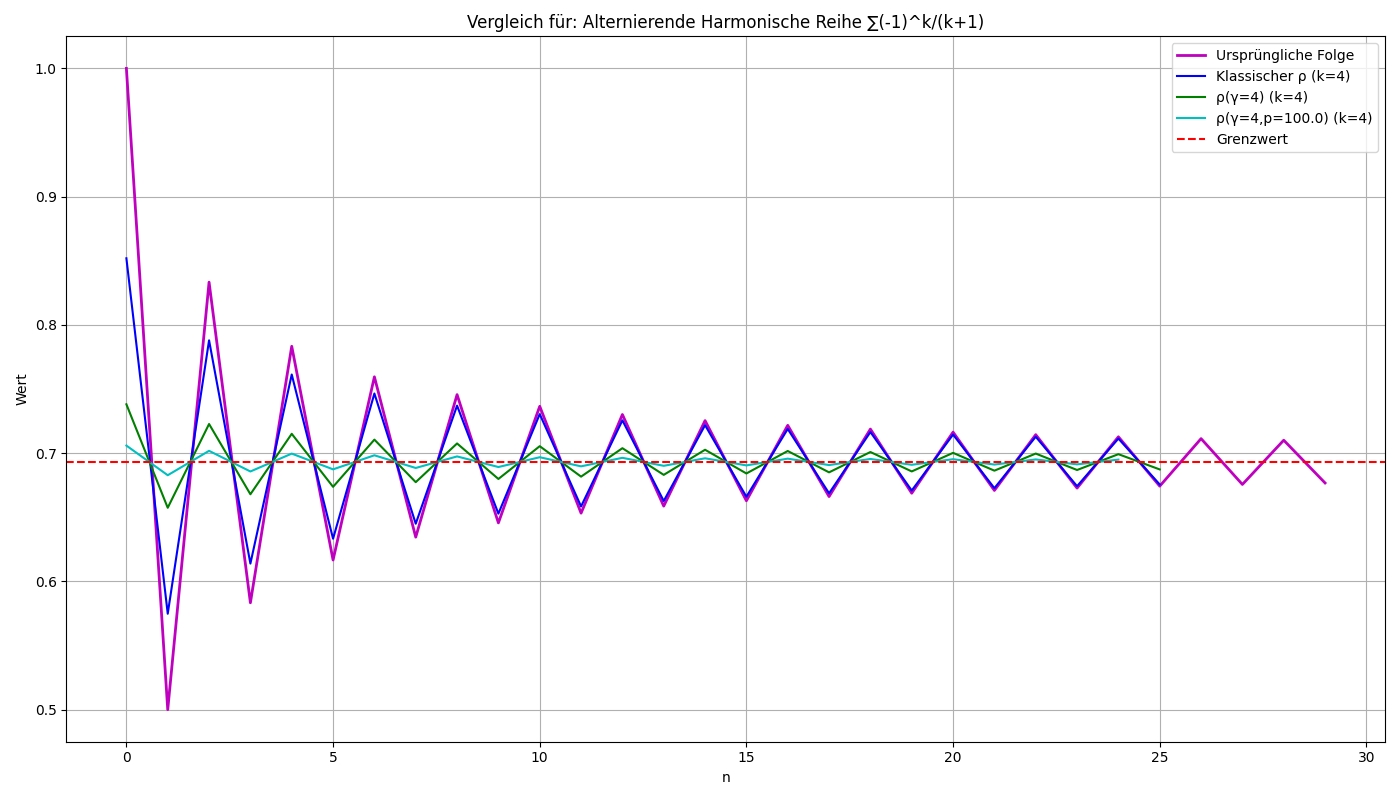
\includegraphics[width=\textwidth]{modi2.png}
In our applications, changing the $\gamma$ parameter yields the coarse improvement, while the parameter $p$ adds no more than $\approx 10^{-6}$.

\newpage
\printbibliography[heading=bibintoc, title={References}]

\end{document}
